\subsection{Carnot Cycle}\label{subsec:Carnot_Cycle}
The \nameref{def:Process} path of the \nameref{def:Carnot_Cycle} is shown in \Cref{fig:Carnot_Cycle}.

\begin{figure}[h!tbp]
  \centering
  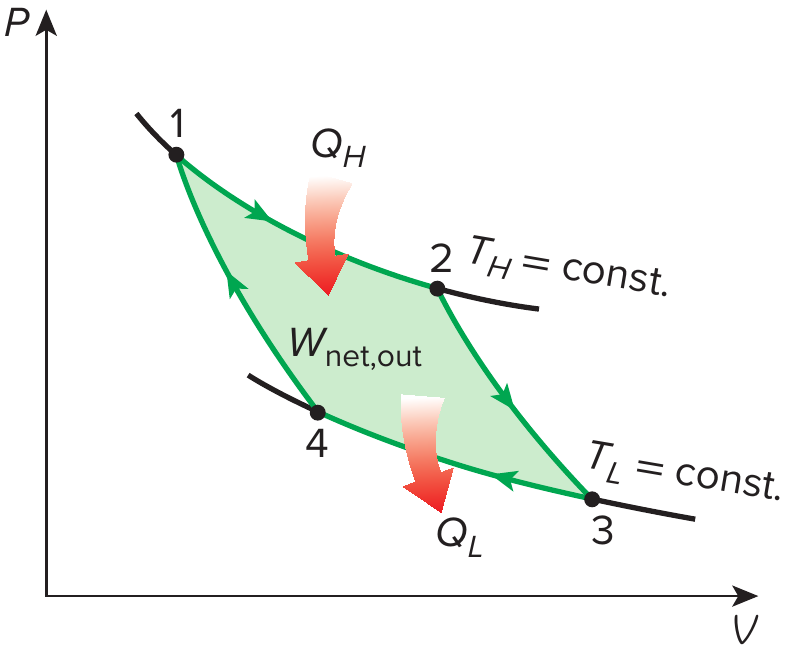
\includegraphics[scale=0.75]{Carnot_Cycle.png}
  \caption{Carnot Cycle (\cite[pg. 252]{ThermoTextbook})}
  \label{fig:Carnot_Cycle}
\end{figure}

\begin{definition}[Carnot Cycle]\label{def:Carnot_Cycle}
  The \emph{Carnot cycle} is a thermodynamically ideal \nameref{def:Cycle}.
  The temperatures $\Temp_{H}$ and $\Temp_{L}$ are isotherms.
  The vertical cases are times when the \nameref{def:System} is perfectly \nameref{def:Adiabatic}, meaning only \nameref{def:Work}, $\Work$, is done.
  The interior of the cycle's process path is the net work done by the \nameref{def:System}.
\end{definition}

If we look at the efficiency of the \nameref{def:Carnot_Cycle}, we see something interesting.
\begin{align*}
  \Efficiency_{C} &= 1 - \frac{\Heat_{Out}}{\Heat_{In}} \\
                  &= 1 - \frac{\Heat_{Out} \propto \Temp_{L}}{\Heat_{In} \propto \Temp_{H}} \\
                  &= 1 - \frac{\Temp_{L}}{\Temp_{H}}
\end{align*}

\begin{equation}\label{eq:Coefficient_of_Performance-Carnot_Cycle}
  \begin{aligned}
    \CoP_{C, HP} &= \frac{1}{1 - \frac{\Heat_{L}}{\Heat_{H}}} \\
    &= \frac{1}{1 - \frac{\Temp_{L}}{\Temp_{H}}} \\
  \end{aligned}
\end{equation}

Because the \nameref{def:Carnot_Cycle} is idealized, we can also run it backwards, making it a refrigerator.
This is seen in \Cref{fig:Carnot_Cycle-Backwards}.

\begin{figure}[h!tbp]
  \centering
  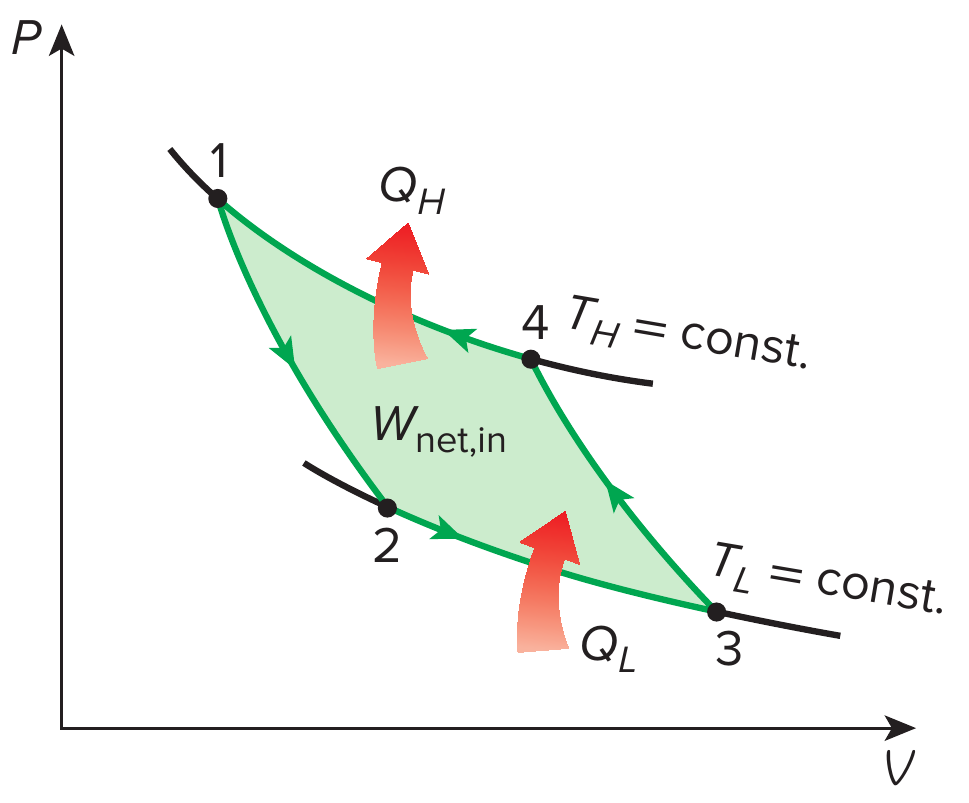
\includegraphics[scale=0.50]{Carnot_Cycle-Backwards.png}
  \caption{Carnot Cycle, in Reverse (\cite[pg. 253]{ThermoTextbook})}
  \label{fig:Carnot_Cycle-Backwards}
\end{figure}

The \nameref{def:Coefficient_of_Performance} for the reversed \nameref{def:Carnot_Cycle} is:
\begin{equation}\label{eq:Coefficient_of_Performance-Carnot_Cycle_Reversed}
  \begin{aligned}
    \CoP_{C, R} &= \frac{1}{\frac{\Heat_{H}}{\Heat_{L}} - 1} \\
    &= \frac{1}{\frac{\Temp_{H}}{\Temp_{L}} - 1} \\
  \end{aligned}
\end{equation}


%%% Local Variables:
%%% mode: latex
%%% TeX-master: "../../MMAE_320-Thermo-Reference_Sheet"
%%% End:
